\section{Architettura}
Lo scopo di questa sezione è di descrivere l'architettura e i design pattern\glosp utilizzati.
\subsection{Design pattern}
\begin{figure}[H]
	\centering
	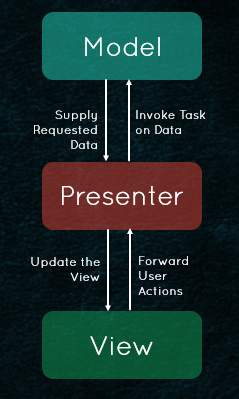
\includegraphics[width=0.3\textwidth]
	{res/images/mvp.png}\\
	\caption{Schema MVP}
	\label{Schema MVP}
\end{figure}
P2PCS implementa il design pattern MVP\glosp seguendo le linee guida fornite da Google\glosp e reperibili al seguente link: \url{https://github.com/googlesamples/android-architecture}.
\newline
\subsubsection{Model}
Contiene i dati che l’applicazione può elaborare e visualizzare. Mette inoltre a disposizione metodi per leggere e modificare tali dati.
In questo progetto fornisce i metodi di lettura e scrittura su Firebase\glo.
Il model è dotato di tre servizi principali, successivamente segmentati in macro-argomenti, che sono:
\begin{itemize}
	\item Authentication
	\item Database
	\item Storage
\end{itemize}
\subsubsection{View}
Rappresenta l’interfaccia utente. Ogni View\glosp disegna sul dispositivo una schermata che permette all’utente di interagire con l’applicazione.
\subsubsection{Presenter}
È il mediatore tra Model\glosp e View\glosp ed elabora i dati del Model\glosp in modo che possano essere visualizzati nella View\glosp e risponde alle richieste dell'utente nella
View\glosp interagendo con il Model. Il Presenter\glosp quindi vuole tenere separate la parte grafica dell'applicazione e la logica di business.

Ogni Activity\glosp quindi sarà composta da una View\glosp e un Presenter\glosp che saranno legati da un contratto che ne definisce le rispettive interfacce.
\begin{figure}[H]
	\centering
	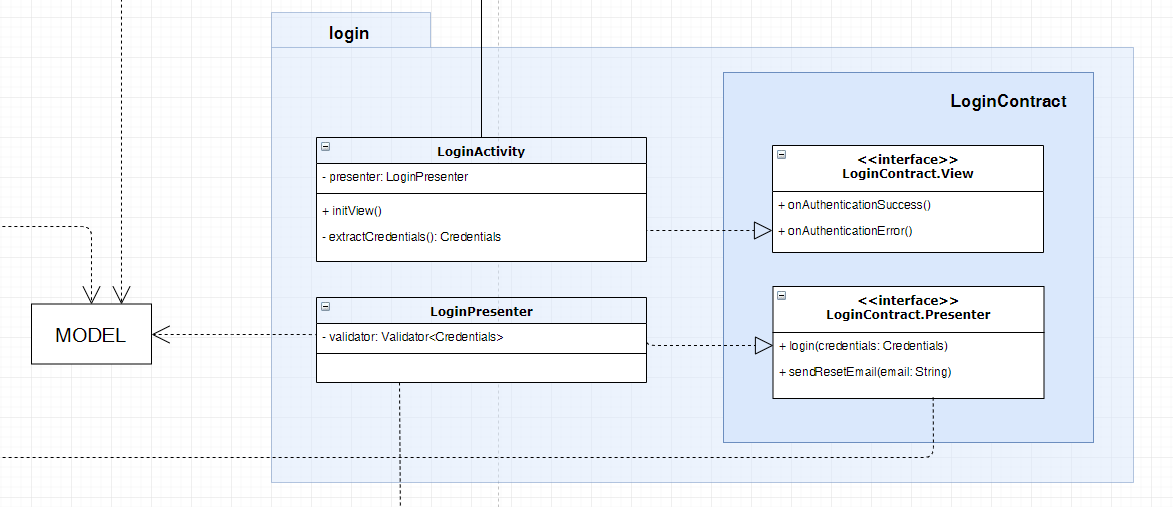
\includegraphics[width=0.9\textwidth]
	{res/images/contratto.png}\\
	\caption{Diagramma d'esempio del Login}
	\label{Schema Login}
\end{figure}
\newpage
\subsection{Directory tree}
\begin{figure}[H]
	\centering
	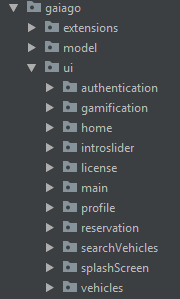
\includegraphics[width=0.3\textwidth]
	{res/images/directorytree.png}\\
	\caption{Directory tree}
	\label{Directory Tree}
\end{figure}
\begin{itemize}
	\item \textbf{extension} contiene classi e funzioni di utilità come la conversione di una data in millisecondi ad una data in formato ddMMyyy;
	\item \textbf{model} contiene i package\glo, classi e interfacce che si occupano della gestione di Firebase\glo;
	\item \textbf{ui} contiene la user interface suddividendola in macro-package.
\end{itemize}
\begin{figure}[H]
	\centering
	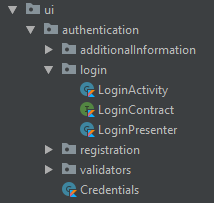
\includegraphics[width=0.3\textwidth]
	{res/images/authentication.png}\\
	\caption{Authentication package}
	\label{Authentication package}
\end{figure}
Ogni macro-package è infine suddiviso in package\glosp che rappresentano le singole funzionalità dell'applicazione, questi sono composti principalmente da View\glosp, Presenter\glosp e Contract\glosp. Alcuni package\glosp possono contenere fragment\glosp aggiuntivi.